% \subsection{Periodo di Validazione e collaudo}
\subsubsection{MQP01 - Indice di Gulpease}
Di seguito sono riportati, attraverso l'uso di una tabella e di diagrammi, i valori rilevati al termine dell'ultimo incremento, tutti i documenti hanno raggiunto il vaolore ottimale.
\begin{table}[H]
    \rowcolors{2}{gray!25}{white}
    \rowcolors{2}{gray!25}{white}
        \renewcommand{\arraystretch}{1.5}
        \begin{tabular}{m{0.4\textwidth}<{\centering}  m{0.25\textwidth}<{\centering}  m{0.25\textwidth}<{\centering} }
            \rowcolor{darkblue}
            \textcolor{white}{\textbf{Documento}}& \textcolor{white}{\textbf{Valore}} & \textcolor{white}{\textbf{Esito}}\\ 

            \textit{NormeDiProgetto-v3.0.0} &
            70 &
            Superato \\

            \textit{PianoDiProgetto-v3.0.0} &
            78 &
            Superato \\

            \textit{PianoDiQualifica-v3.0.0} &
            75 &
            Superato \\

            \textit{AnalisiDeiRequisiti-v3.0.0} &
            90 &
            Superato \\
            
            \textit{Glossario-v3.0.0} &
            82 &
            Superato \\
            \textit{SpecificaArchitetturale-v2.0.0} &
            85 &
            Superato \\
            \textit{ManualeUtente-v2.0.0} &
            82 &
            Superato \\

            \textit{VerbaleEsterno-2022.06.07} &
            72 &
            Superato \\
          
            \textit{VerbaleInterno-2022.06.06} &
            75&
            Superato \\
    \end{tabular}
    \caption{Validazione e collaudo: MQP01 - Indice di Gulpease}
\end{table}
\begin{figure}[H]
    \centering
    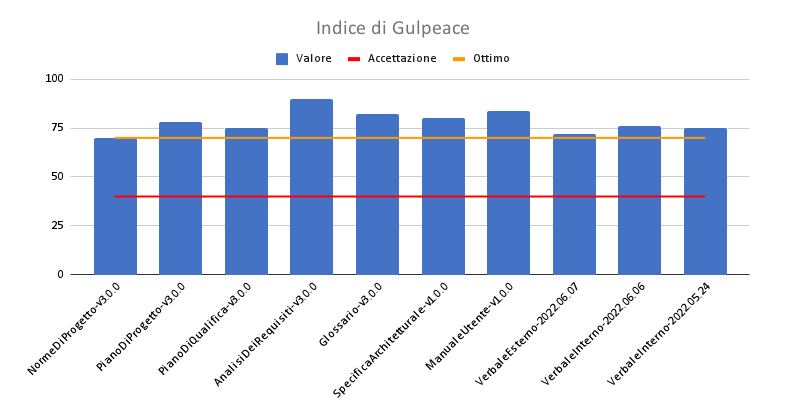
\includegraphics[scale=0.50]{Sezioni/images/last_prodotto/Indice_di_Gulpeace.png}
    \caption{Validazione e collaudo: MPC02 - BCWS}
\end{figure}
\subsubsection{MQP02 - Profondità di una gerarchia}
\begin{figure}[H]
    \centering
    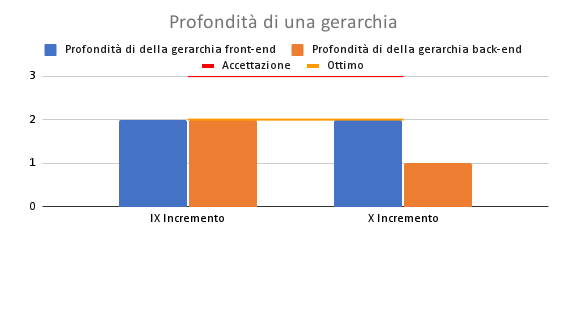
\includegraphics[scale=0.50]{Sezioni/images/last_prodotto/Profondita_di_una_gerarchia.png}
    \caption{Validazione e collaudo: MQP02 - Profondità di una gerarchia}
\end{figure}
\subsubsection{MQP03 - Numero parametri per metodo}
\begin{figure}[H]
    \centering
    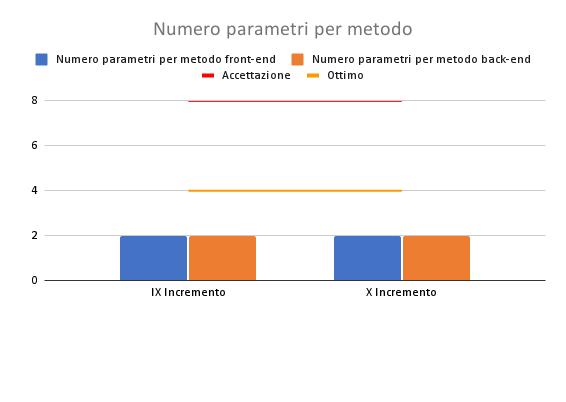
\includegraphics[scale=0.50]{Sezioni/images/last_prodotto/Numero_parametri_per_metodo.png}
    \caption{Validazione e collaudo: MQP03 - Numero parametri per metodo}
\end{figure}
\subsubsection{MQP04 - Code coverage}
\begin{figure}[H]
    \centering
    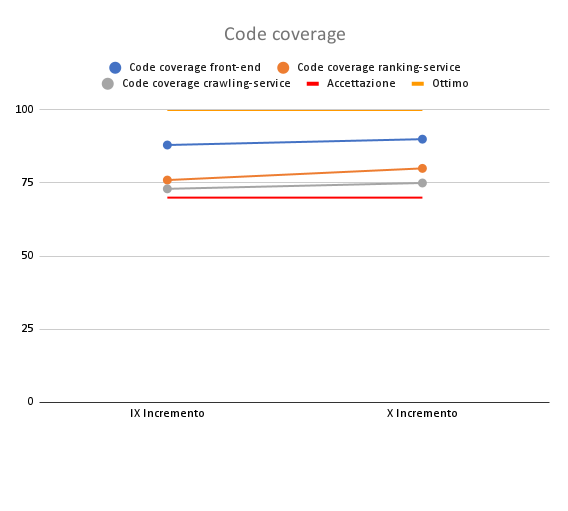
\includegraphics[scale=0.50]{Sezioni/images/last_prodotto/Code_coverage.png}
    \caption{Validazione e collaudo: MQP04 - Code coverage}
\end{figure}
\subsubsection{MQP05 - Percentuale requisiti obbligatori soddisfatti}
Nella fase finale del progetto il gruppo è riuscito a soddisfare tutti requisiti obbligatori.
\begin{figure}[H]
    \centering
    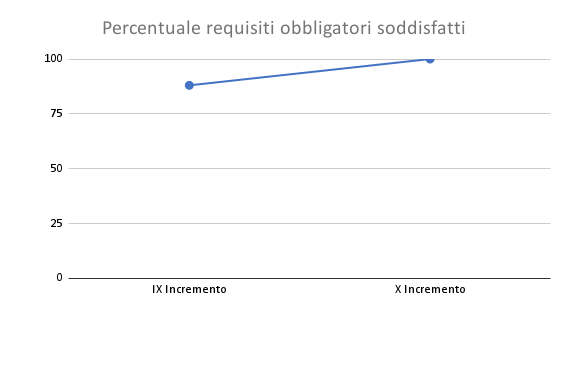
\includegraphics[scale=0.50]{Sezioni/images/last_prodotto/Percentuale_requisiti_obbligatori_soddisfatti.png}
    \caption{Validazione e collaudo: MQP05 - Percentuale requisiti obbligatori soddisfatti}
\end{figure}
\subsubsection{MQP06 - Complessità ciclomatica}
Il gruppo durante ultima fase è riuscito a raggiunge il valore ottimale complessità ciclomatica, grazie all'implementazione della nuova funzionalità.
\begin{figure}[H]
    \centering
    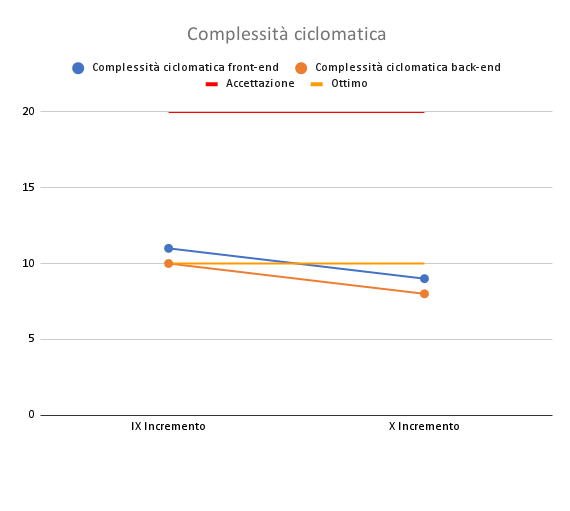
\includegraphics[scale=0.50]{Sezioni/images/last_prodotto/Complessita_ciclomatica.png}
    \caption{Validazione e collaudo: MQP06 - Complessità ciclomatica}
\end{figure}
\subsubsection{MQP07 - Numero di bug}
Rispetto ai precedenti incrementi nelle ultime due fasi del progetto, il gruppo è riuscito ad azzerare il numero di bug.
\begin{figure}[H]
    \centering
    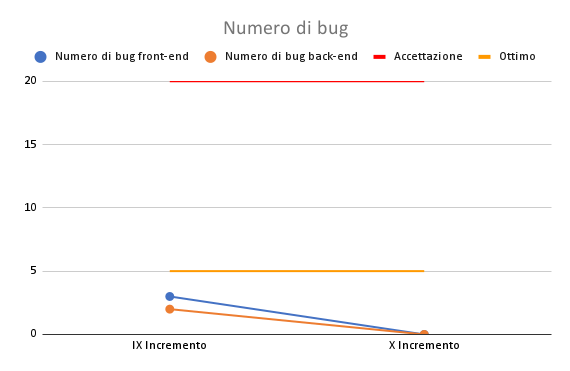
\includegraphics[scale=0.50]{Sezioni/images/last_prodotto/Numero_di_bug.png}
    \caption{Validazione e collaudo: MQP07 - Numero di bug}
\end{figure}
\subsubsection{MQP08 - Numero di Code smell}
\begin{figure}[H]
    \centering
    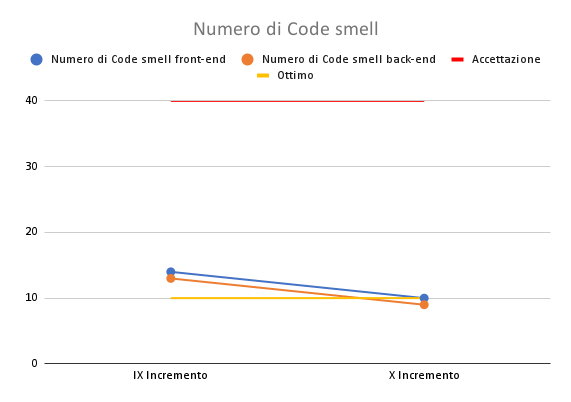
\includegraphics[scale=0.50]{Sezioni/images/last_prodotto/Numero_di_Code_smell.png}
    \caption{Validazione e collaudo: MQP08 - Numero di Code smell}
\end{figure}
\subsubsection{MQP09 - Linee di Commento per Linee di Codice}
Nell'ultimo incremento il progetto ha raggiunto il valore di accettazione richiesto per i linee di commento per linee di codice.
\begin{figure}[H]
    \centering
    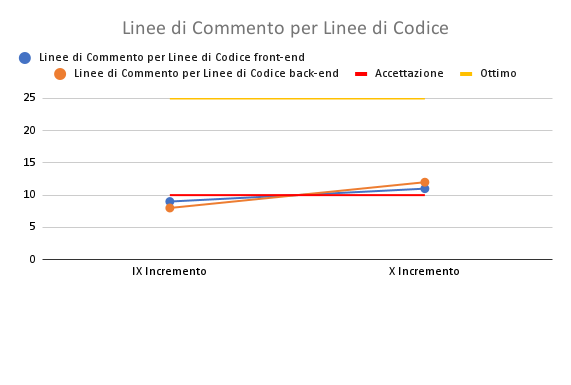
\includegraphics[scale=0.50]{Sezioni/images/last_prodotto/Linee_di_Commento_per Linee_di_Codice.png}
    \caption{Validazione e collaudo: MQP09 - Linee di Commento per Linee di Codice}
\end{figure}
\subsubsection{MQP10 - Branch Coverage}
\begin{figure}[H]
    \centering
    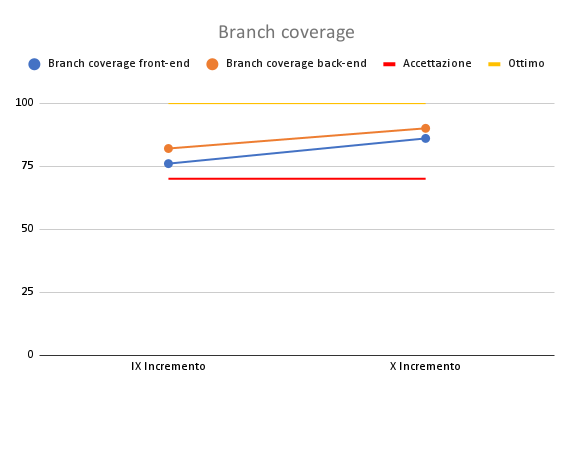
\includegraphics[scale=0.50]{Sezioni/images/last_prodotto/Branch_coverage.png}
    \caption{Validazione e collaudo: MQP10 - Branch Coverage}
\end{figure}
\subsubsection{MQP11 - Successo di test}
\begin{figure}[H]
    \centering
    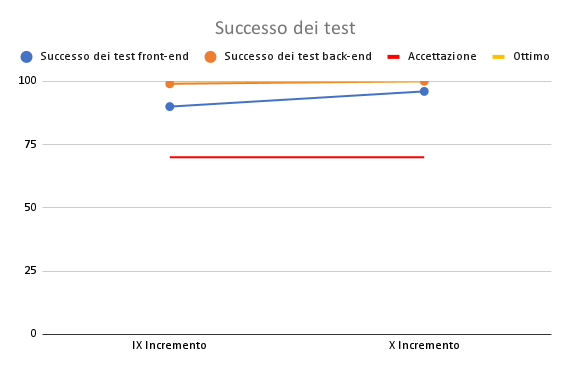
\includegraphics[scale=0.50]{Sezioni/images/last_prodotto/Successo_dei_test.png}
    \caption{Validazione e collaudo: MQP11 - Successo di test}
\end{figure}
\subsubsection{MQP12 - Numero di vulnerabilità}
\begin{figure}[H]
    \centering
    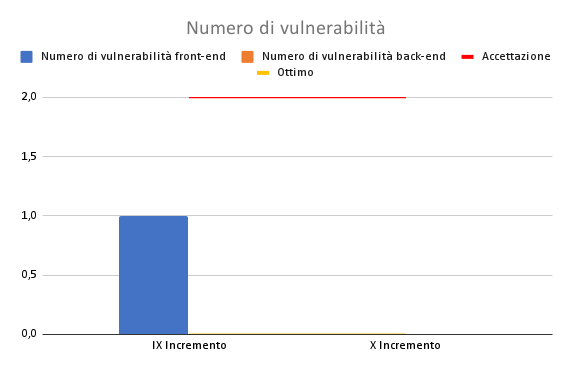
\includegraphics[scale=0.50]{Sezioni/images/last_prodotto/Numero_di_vulnerabilita.png}
    \caption{Validazione e collaudo: MQP12 - Numero di vulnerabilità}
\end{figure}

\subsubsection{MTS1 - Test eseguiti in rapporto ai requisiti}
\begin{table}[H]
    \rowcolors{2}{gray!25}{white}
    \renewcommand{\arraystretch}{1.5}
    \begin{tabular}{ m{0.4\textwidth}<{\centering}  m{0.2\textwidth}<{\centering}  m{0.2\textwidth}<{\centering} m{0.2\textwidth}<{\centering} }
        \rowcolor{darkblue}
        \textcolor{white}{\textbf{Incremento}} &\textcolor{white}{\textbf{Valore calcolato}}& \textcolor{white}{\textbf{Valore ottimo}} & \textcolor{white}{\textbf{Valore tollerato}}\\ 
        
        IX Incremento & 
        100\% &
        100\% &
        100\% \\

        X Incremento & 
        100\% &
        100\% &
        100\% \\

    \end{tabular}
    \caption{Validazione e collaudo: MTS1 - Test eseguiti in rapporto ai requisiti}
\end{table}

\subsubsection{MTS1 - Percentuale test passati}
\begin{table}[H]
    \rowcolors{2}{gray!25}{white}
    \renewcommand{\arraystretch}{1.5}
    \begin{tabular}{ m{0.4\textwidth}<{\centering}  m{0.2\textwidth}<{\centering}  m{0.2\textwidth}<{\centering} m{0.2\textwidth}<{\centering} }
        \rowcolor{darkblue}
        \textcolor{white}{\textbf{Incremento}} &\textcolor{white}{\textbf{Valore calcolato}}& \textcolor{white}{\textbf{Valore ottimo}} & \textcolor{white}{\textbf{Valore tollerato}}\\ 
        
        IX Incremento & 
        100\% &
        100\% &
        85\% \\

        X Incremento & 
        100\% &
        100\% &
        85\% \\

    \end{tabular}
    \caption{Validazione e collaudo: MTS2 - Percentuale test passati}
\end{table}